
Somewhat surprisingly, Swarm's network layer can serve as an efficient  communication platform with exceptionally strong privacy properties. This chapter is an attempt to define a comprehensive set of primitives that serve as building blocks for a base layer communication infrastructure covering the full range of communication modalities including real time anonymous chat, sending and receiving messages from previously not connected, potentially anonymous senders, mailboxing for asynchronous delivery, long term notifications and  publish/subscribe interfaces. 


\section{Swarm feeds and mutable resource updates \statusyellow}\label{sec:feeds}

\yellow{WIP: rewritten, review needed}

Feeds are a unique feature of swarm. They constitute the primary use case for single-owner chunks. Feeds can be used for versioning revisions of a mutable resource, indexing sequential updates to a topic, publish the parts to streams, or post consecutive messages in a communication channel to name but a few. Feeds implement persisted pull-messaging and can also be interpreted as a pub-sub system.
First, in \ref{sec:feed-chunks}, we introduce how feeds are composed of single-owner chunks with an indexing scheme, the choice of which we discuss in  (\ref{sec:indexing-schemes}. In \ref{sec:feed-integrity}, we analyse why feed integrity is relevant and how it can be verified and enforced. \ref{sec:epoch-based-feeds} describe \gloss{epoch-based feeds} which provide feeds with sporadic updates a way to be searched. Finally, in \ref{sec:feed-as-channel}, we show how feeds are used as an outbox to store subsequent messages in a communication channel.


\subsection{Feed chunks \statusyellow}\label{sec:feed-chunks}

A feed chunk is a single-owner chunk with the associated constraint that the identifier is composed as the hash of a \gloss{feed topic} and a \gloss{feed index}. The topic is a 32-byte arbitrary byte array, this is typically the keccak256 hash of one or more human readable strings specifying the topic and optionally the subtopic of the feed, see figure \ref{fig:feed-chunk}. 


\begin{figure}[htbp]
\centering
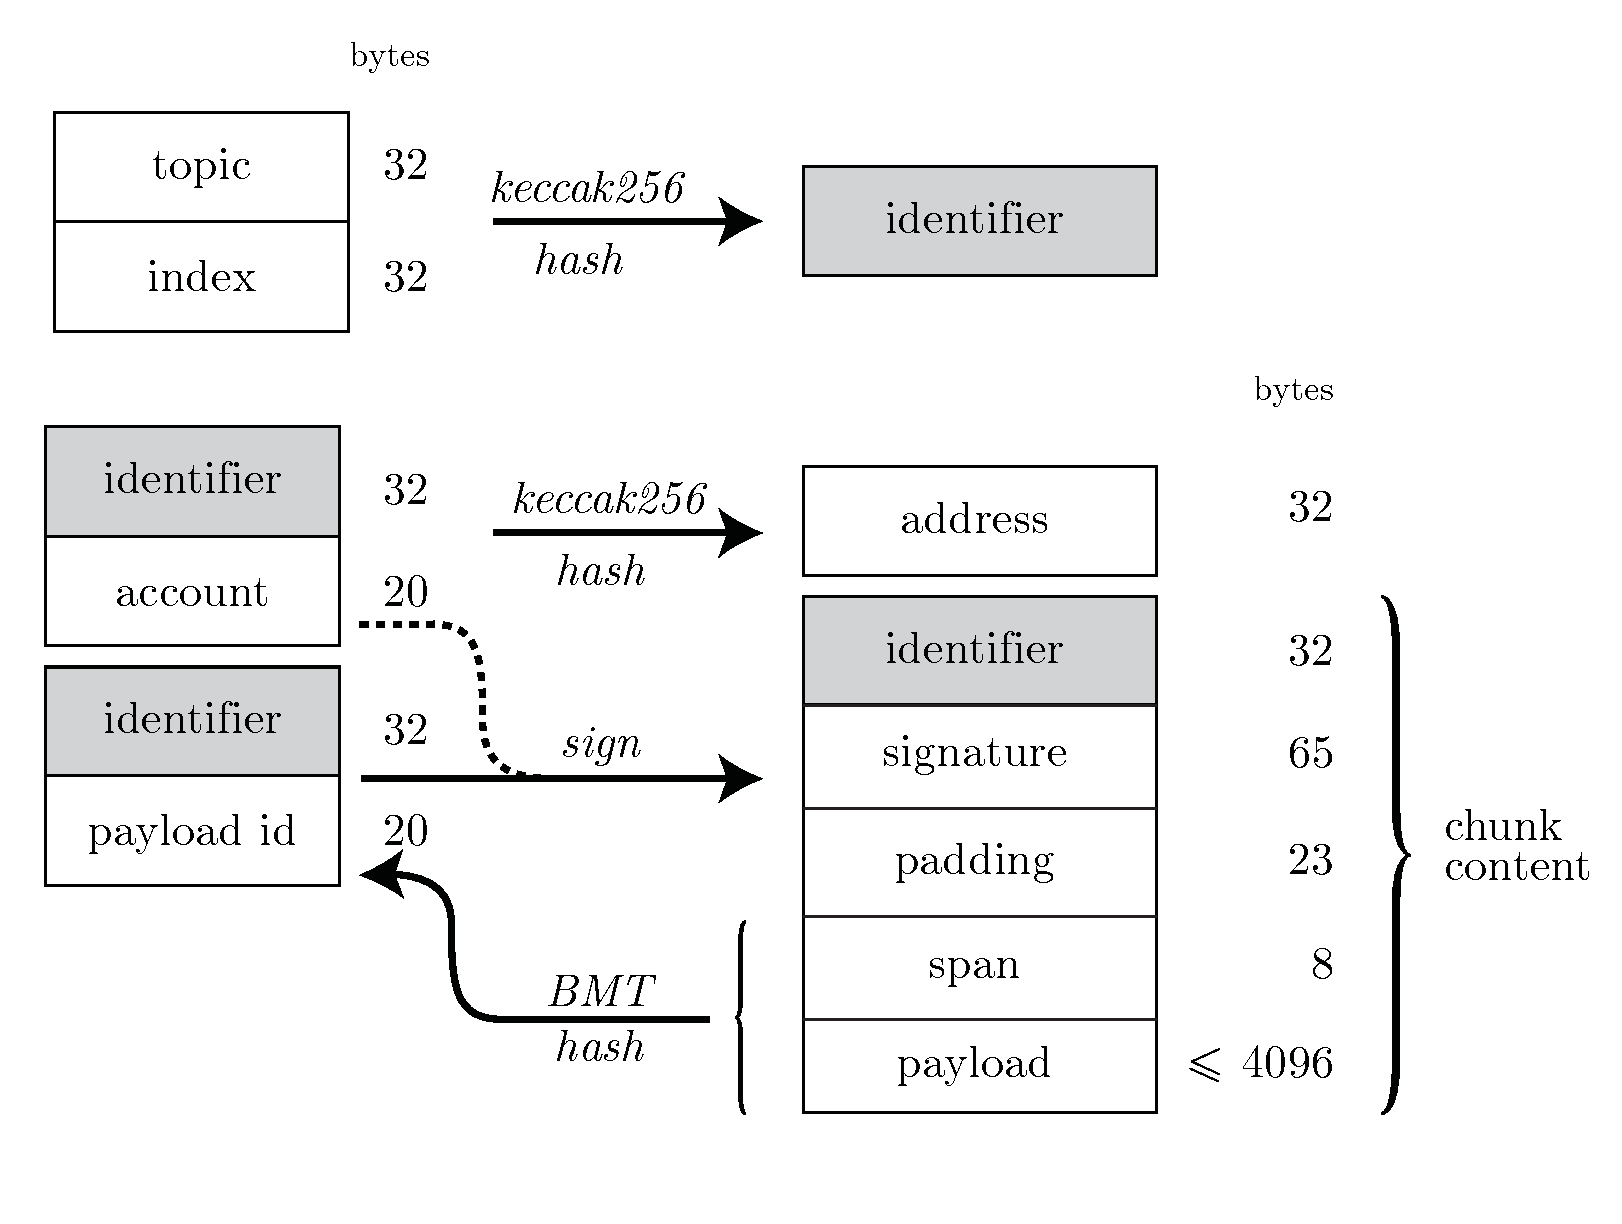
\includegraphics[width=\textwidth]{fig/feed-chunk.pdf}
\caption[Feed chunk \statusred]{Feed chunk}
\label{fig:feed-chunk}
\end{figure}

The index can take various forms defining various types of feeds discussed in this section: (1) simple feeds use incremental integers as index (\ref{sec:indexing-schemes}); (2)  \gloss{epoch-based feeds} use epoch ID (\ref{sec:epoch-based-feeds}); and (3) private channel feeds use the nonces generated with a \gloss{double ratchet} key chain.  (\ref{sec:feed-as-channel}).
The unifying property of all feed types is that publisher (owner) and consumer both know the \gloss{indexing scheme}. 

Publishers are the single owners of feed chunks and are the only ones able to post updates to their feed. Posting an update requires (1) constructing the identifier from the topic and the correct index and (2) signing it with the hash of the arbitrary content of the update. Since the identifier designates an address in the owner's subspace of addresses, this signature effectively assigns the payload to this address (see \ref{sec:single-owner-chunks}). 

Conversely, users  can consume a feed by retrieving the chunk by its address. Retrieving an update requires the consumer to construct the address from the owner's public key and the identifier. To calculate the identifier they need the topic and the appropriate index. For this they need to know the indexing scheme. 

Feeds enable Swarm users to represent a sequence of content updates. The content of  the update is the payload that the feed owner signs against the identifier. The payload can be a swarm reference.

\subsection{Indexing schemes \statusyellow}\label{sec:indexing-schemes}

Different types of feeds require different indexing schemes and different lookup strategies. In what follows, we introduce a few largely independent dimensions in which feeds can be categorised and which appear relevant in making a choice.


The actual indexing scheme used or even whether there is one (i.e., if the single owner chunk is a feed chunk at all) is left unrevealed in the structure of a feed chunk. As this information is not needed for the validation of the single-owner chunk by forwarding nodes, having the subtype explicit in the structure would leak  information unnecessarily. 

\subsubsection{Update semantics}

Updates of a feed can have three distinct semantics defining three subtypes of feeds. 
Revisions or mutable resource updates are \emph{substitutive}, series updates are \emph{alternative}, while partition updates are \emph{accumulative}. 

Feeds that represent revisions of the same semantic entity are called \gloss{mutable
resource updates}. These resources mutate because the underlying semantic entity changes such as versions of your CV or the resource description becomes more elaborate like the wikipedia entry about a Roman emperor. Users will typically be interested in the latest update of such resources, past versions having only historical significance. 

A series of content connected by a common thread, theme or author such as status updates on social media, a person's blog posts or blocks of a blockchain can also be represented with feeds called \gloss{series}.
The updates in a series are interpreted as alternative and independent instantiations or episodes manifesting in temporal sequence. 

Finally, there are \gloss{partitions} expressed as feeds, updates of which are meant to be accumulated or added to earlier ones, for instance, parts of a video stream. These mainly differ from series in that the feed updates are not interpretable on their own and the temporal sequence may represent processing order corresponding to some serialisation of the structure of the resource rather than temporal succession. When such a feed is accessed, accumulation of all the parts may be necessary even for the integrity of the represented resource.

If subsequent updates of a feed include a reference to a data structure indexing the previous updates (e.g., a key-value store using the timestamp for the update or simply the root hash of the concatenation of update content), then the \gloss{lookup strategy} in all three cases reduces to looking up the latest update.

\subsubsection{Update frequency}

There are \gloss{sporadic feeds} with irregular asynchronicities, i.e., updates can have unpredictable gaps  and also \gloss{periodic feeds} with updates published at regularly recurring intervals.

We also talk about \gloss{real-time feeds}, where the update frequencies may not be regular but show variance within the temporal span of real-time human interaction, i.e., punctuated by intervals in the second to minute range.

\subsubsection{Subscriptions}

Feeds can be interpreted as \gloss{pub-sub systems} with persistence enabling asynchronous pulls. In what follows we analyse how the implementation of subscriptions to feeds as pub/sub is effected by the choice of indexing scheme.

In order to cater for subscribers to a feed, updates need to be tracked. If we know the  latest update, periodic polling needs to be used to fetch the subsequent update. 
If the feed is periodic one can start polling after a known period. Alternatively, if the feed updates are frequent enough (at most a 1-digit integer orders of magnitude rarer than the desired polling frequency), then polling is also feasible.
However, if the feed is sporadic, polling may not be practical and we better resort to push notifications (see \ref{sec:trojan} and \ref{sec:update-notification-requests}).

If we missed out on polling for a period of time due to being offline, or just created the subscription, we can also rely on push notifications or use a \gloss{lookup strategy}. 

To look up partitions is not a problem since we need to fetch and accumulate each update so just the strategy of iterating over the  successive indexes cannot be improved.
For periodic feeds, we can just calculate the index for the current time, hence asynchronous access is efficient and trivial. 
Looking up the latest version of a sporadically updated feed, however, necessitates some search and hence 
will benefit from \gloss{epoch-based indexing}.



\subsubsection{Aggregate indexing}

A set of sporadic feeds can be turned into a periodic one using \gloss{feed aggregation}. Imagine a multi-user forum like reddit where each registered participant would publish comments on a post using sporadic feeds. In this scenario it is not practical for each user to monitor the comment feed of other users and search their sporadic feeds for updates in order to retrieve all the comments on the thread. It is worth doing it once though for all users. Indexers do exactly that and aggregate everyone's comments in an index, a data structure the root of which can now be published as a periodic feed, see figure \ref{fig:feed-aggregation}. The period can be chosen to give a real-time feed experience; even if the rate of change does not justify it, i.e., some updates will be redundant, the cost amortises over all users that use the aggregate feed and therefore is economically sustainable. 

\begin{figure}[htbp]
\centering
\caption[Feed aggregation \statusred]{Feed aggregation}
\label{fig:feed-aggregation}
\end{figure}

Such a service can be provided with arbitrary levels of security, yet trustlessly without resorting to reputation. Using consensual data structures for the aggregation, incorrect indexes can be proved using cheap and compact inclusion proofs (see \ref{sec:files}) and therefore any challenge relating to correctness can be evaluated on chain. The threat of losing their deposit in case of an unrefuted challenge acts as a strong incentive for providers to maintain quality of service.


\subsection{Integrity \statusyellow}\label{sec:feed-integrity}

We say that a feed has \emph{integrity} if each of its updates has integrity, i.e., the update is unambiguous. Formally this means that for each index, the respective feed identifier is only ever assigned to a single payload. Incidentally this also implies that the corresponding feed chunk has integrity. As discussed in \ref{sec:single-owner-chunks}, this is a prerequisite for consistent retrieval. 
If the payloads of the successive updates are imagined as blocks of a blockchain, then the criterion of integrity means that owners must not fork their chain. 

The integrity of a feed can only be guaranteed by the owner. But can in be checked or enforced? Owners can commit to the integrity of their feeds by staking a deposit on the blockchain which they stand to lose if they are found to double sign on an update. Eventhough this may give a strong disincentive to fork a feed for long-term benefits, by itself, it is unable to give sufficient guarantees to consumers of the feed with respect to  integrity. 

\subsubsection{Authoritative version history}

Mutable resource update feeds track versions pretty much the same way as the Ethereum Name Service does.  
When the owner consolidates a version, they want to register the content address of the current version. In order to guarantee that there is no dispute over history, the payload needs to incorporate the previous payload hash. This requires the payload to be a composite structure. If we want the payload to just be a manifest or manifest entry, so it can be rooted to a path matching a URL, or directly displayed, it  is not possible. Also if the feed content is not a payload hash, then ENS registers a payload hash but the chunk may not exist on swarm, so then the semantics of ENS is violated.

An indexing scheme which incorporates the previous payload hash into the subsequent index behaves like a blockchain in that it expresses the owner unambiguous commitment to history and any consumer reading and using it expresses their acceptance of such history. 
Looking up such feeds is only possible by retrieving each update since the last  known one. The address is that of the update chunk so registering the update address both guarantees historic integrity yet preserves ENS semantics that the registered address is a swarm reference to a chunk.
Such feeds implement an \gloss{authoritative version history}, i.e., a secure audit trail of the revisions of a mutable resource. 

\subsubsection{Real-time integrity check}

A deterministically indexed feed enables a \gloss{real-time integrity check}. In the context of feeds that represent blockchains (ledgers/side-chains), integrity translates to non-forking or unique chain commitment. The ability to enforce this real-time allows fast and secure definitions of transaction finality. 

We illustrate this with an example of off-chain p2p payment network where each node's locked up funds are allocated to a fixed set of creditors (see more detail in \cite{ethersphere2019swap}). Creditors of the node need to check the correctness of reallocations, i.e., the total increases are covered by countersigned decreases. 
If a debitor keeps publishing a deposit allocation table for an exhaustive list of creditors, by issuing two alternatives to targeted creditors the debitors can orchestrate a double spend. Conversely, certainty in the uniqueness of the allocation table allows the creditor to conclude finality.

We claim that using swarm feeds, this uniqueness constraint  can be checked real time.

The insight here is that it is impossible to meaningfully control the responses to a single-owner chunk request: There is no systematic way to respond with particular versions to particular requestors even if the attacker controls the entire neighbourhood of the chunk address.%
%
\footnote{If the chunks are uploaded using the same route, the chunk that comes later will be rejected as already known. If the two chunks originate from different addresses in the network, they might both end up in their local neighbourhood. This scenario will result in inconsistent retrievals depending on which node the request ends up with.}
%
This is the result of the ambiguity of the originator due to forwarding Kademlia. Let us imagine that the attacker, with some sophisticated traffic analysis, has the chance of $1/n$ (asymptotic ceiling) to identify the originator of the request and give a differential response. Sending multiple requests from random addresses, however, one can test integrity and require consistent response for finality. The chance that the attacker can give a consistent differential response to a creditor testing with $k$ independent requests is $1/n^k$. With linear bandwidth cost in $k$, we can achieve expontential degrees of certainty about the uniqueness of an update. If a creditor finds consistency, it concludes that there is no alternative allocation table.


By requiring the allocation tables to be disseminated as feed updates, we can leverage permissionlessness, availability and anonymity to enforce feed integrity. If the feed is a blockchain-like ledger, a real-time integrity check translates to fork finality. 


\subsection{Epoch-based 
indexing \statusyellow}\label{sec:epoch-based-feeds}

\yellow{}

In order to use single owner chunks to implement feeds  with flexible update frequency, we introduce \gloss{epoch-based feeds}, an indexing scheme where the single-owner chunk's identifier incorporates anchors related to the time of publishing. In order to find the latest update, we introduce
an adaptive lookup algorithm. 

\subsubsection{Epoch grid}

An \gloss{epoch} represents a concrete time period starting at a specific point in time, called the \gloss{epoch base time} and has a specific length.  
Period lengths are expressed as powers of 2 in seconds. The shortest period is $2^0 = 1$ second,  the longest is $2^{31}$ seconds. 

An \gloss{epoch grid} is the arrangement of epochs where rows (referred to as levels) represent alternative partitioning of time into various disjoint epochs with the same length. Levels are indexed by the logarithm of the epoch length putting level 0 with 1 second epoch length at the bottom by convention, see figure \ref{fig:epoch-grid}.

\begin{figure}[htbp]
\centering
\includegraphics[width=\textwidth]{fig/feeds/02.png}
\caption[Epoch grid showing the first few updates of an epoch-based feed \statusgreen]{Epoch grid showing the first few updates of an epoch-based feed. Epochs occupied are marked in yellow and are numbered to reflect the order of updates they represent. }
\label{fig:epoch-grid}
\end{figure}

When representing a epoch-based feed in an epoch grid, each updates is assigned to a different epoch in the grid based on  their timestamp. In particular, an update is mapped to the longest free epoch that includes the timestamp. This structure gives the series of updates a contiguous structure which allows for easy search. The contiguity requirement implies that knowing the epoch of the previous update, a subsequent update is mapped to an epoch unambiguously.


To identify a specific epoch, we need to know both the epoch base time and the level. This pair is called \gloss{epoch reference}. To calculate the epoch base time of any given instant in time $t$ at a particular level $l$, we are dropping the $l$ least significant bits of $t$. 
The level requires one byte, and the epoch base time (using linux seconds)  4 bytes so the epoch reference can be serialised in 5 bytes. 
The epoch reference of the very first update of any epoch-based feed is always the same.

\subsubsection{Mapping epochs to feed update chunks}

Feed updates can then be mapped to feed chunks using the serialised epoch reference as the \gloss{feed index}. The topic of the feed hashed together with the index results in the feed identifier used in constructing the single owner chunk that expresses the feed chunk. 

To determine the epoch in which to store a subsequent update, the publisher needs to know where they stored the previous update. If the publisher cannot keep track of this, they can always use the algorithm to find their last update.



\subsubsection{Lookup algorithm}

When consumers retrieve feeds, they typically want to look up the state of the feed at a particular time (historical lookup), or want to find the latest update.

If historical lookups based on a \emph{target} time is required, the update can incorporate a data structure mapping timestamps to states. In such cases finding any update later than the target can be used to deterministically look up the state at an earlier time. 

If no such index is available, historical lookups need to find the shortest filled epoch whose timestamp is earlier than the target. 


To select the best starting epoch to walk our grid, we have to assume the worst case, which is that the resource was never updated after we last saw it. If we don't know when the resource was last updated, we assume 0 as the "last time" it was updated.

We can guess a start level as the position of the nonzero bit of $\mathit{lastUpdate}\xor \mathit{NOW}$ counting from the left. The bigger the difference among the two times (last update time and now), the higher the level will be.

In \ref{sec:epoch-based-feeds-appendix}, we walk the reader through an example.

\subsection{Real-time data exchange \statusyellow}\label{sec:feed-as-channel}

Feeds can be used to represent a communication channel, i.e., the outgoing messages of a persona. Such a feed called \gloss{outbox feed} can be created for  email-like  communication or instant messaging or the two combined. For email-like asynchronicities, \gloss{epoch-based indexing} can be used while for instant messaging only, best to use deterministic sequence indexing. 
In group chat or group email, confidentiality is handled by using access control trie over the data structure indexing each party's contribution to the thread. Communication clients can retrieve each group member's feed relating to a thread and merge their timelines for rendering. 

Even forums can be implemented with such an outbox mechanism, however, above a certain number of registered participants, aggregating all outboxes on the client side becomes impractical and may require index aggregators.

\subsubsection{Two-way private channels}
 
Private two-party communication can also be implemented using outbox feeds, see figure \ref{fig:feeds-as-channel}. The parameters of such feeds are set as part of an initial key exchange or registration protocol (see \ref{sec:pss-key-exchange}) which ensures that the parties consent on the indexing scheme as well as the encryption used. 


\begin{figure}[h!]
  \centering
  \caption[Swarm feeds as outboxes \statusred]{Swarm  feeds as outboxes for private communication}
\label{fig:feeds-as-channel}
\end{figure}


The real-time series feed used for instant messaging ought to have an indexing scheme with deterministic continuations for at least few updates ahead. This enables sending retrieve requests for future updates ahead of time, i.e., during or even prior to processing the previous messages. When such retrieve requests arrive at the nodes whose address is closest to the requested update address, the chunk will obviously not be found as the other party has not sent them yet. However, even these storer nodes are incentivised to keep retrieve requests alive until they expire (see the argument in \ref{sec:retrieval}). This means that up till the end of their time-to-live setting (30 seconds), requests behave as subscriptions: the arrival of the update chunk triggers the delivery response to the open request as if it was the notification sent to the subscriber. This reduces the expected message latency down to less than twice the average time of one-way forwarding paths, see figure \ref{fig:outbox-feed-latency}). 


\begin{figure}[htbp]
\centering
\caption[Advance requests for future updates \statusred]{Advance requests for future updates}
\label{fig:outbox-feed-latency}
\end{figure}


\subsubsection{Post-compromise security}

A key management solution called \gloss{double ratchet} is the de-facto industry standard used for encryption in instant messaging.
It is customary to use the \gloss{extended triple Diffie--Hellmann Key Exchange} (\gloss{X3DH}) to establish the initial parameters for the double ratchet key chains (see \ref{sec:pss-key-exchange}).

Double ratchet combines a ratchet based on a continuous key-agreement protocol with a ratchet based on key-derivation function \cite{perrin2016double}. This scheme can be generalised \cite{alwen2019double} and understood as a combination of well-understood primitives and shown to provide  (1) forward secrecy, (2) backward secrecy,%
%
\footnote{Also known as future secrecy or post-compromise security.}
%
and (3) immediate decryption and message loss resilience.

On top of the confidentiality due end-to-end encryption, swarm offers further resistance  to attacks. Due to forwarding Kademlia, the sender is ambiguous and deniable. Due to  normal push-sync and  pull-sync traffic, messages are also obfuscated. To make it really hard for an attacker, the sequence of indexes can also provide \gloss{future secrecy} if we add more key chains to the double ratchet machinery. Beside root, sending and receiving encryption key chains, we would need to introduce two more: outgoing and incoming \gloss{outbox index key chains}, see figure \ref{fig:double-ratchet-for-feeds}. As a result of this measure the underlying communication channel  is obfuscated, i.e., intercepting an outbox update chunk and knowing its index, reveals nothing about previous or subsequent outbox update indexes making subsequent messages very difficult and costly to monitor or intercept.

In \ref{sec:feed-integrity}, we used factoring in the payload hash into the indexing scheme to achieve non-mergeability of chains (unambiguous history). Inspired by this, we propose also to factor in the payload hash into the subsequent feed update index. This results in the additional property called \emph{RECOVER-security},  which, intuitively, ensures that once an adversary manages to forge a message from A to B, then no future message from A to B will  be  accepted  by B.
This is guaranteed if the authenticity of A's  messages to B affects the subsequent \gloss{feed index}. If there is a mismatch (one of the messages was forged), messages will be looked up at the wrong address and therefore communication channel will be abandoned and a new one is initiated. We believe that such a communication channel is virtually a zero-leak solution for real-time messaging.


\begin{figure}[htbp]
\centering
\caption[Future secrecy for update addresses \statusred]{Future secrecy for update addresses}
\label{fig:double-ratchet-for-feeds}
\end{figure}



\section{Pss: direct push messaging with mailboxing\statusgreen}\label{sec:pss}

\green{}

This section introduces \emph{pss}, Swarm's direct node-to-node push messaging solution. 
Functionalities of and motivation for its existence are playfully captured by alternative resolutions of the term:

\begin{itemize}
\item \emph{postal service on Swarm} -- Delivering messages if recipient is online or depositing for download if not.
\item \emph{pss is bzz whispered} -- Beyond the association to Chinese whispers, it surely carries the spirit and aspiration of Ethereum Whisper.%
%
\footnote{Whisper is a gossip-based dark messaging system, which is no longer developped. It never saw wide adoption due to its (obvious) lack if  scalability. Whisper, alongside Swarm and the Ethereum blockchain, was the communication component of the holy trinity, the basis for Ethereum's original vision of web3.}
%
pss piggy-backs on Swarm's \gloss{distributed storage} for chunks and hence inherits full incentivisation for relaying and persistence. At the same time it borrows from whisper's crypto, envelope structure and API.
\item \emph{pss! instruction to hush/whisper} -- Evokes the effort to not disclose information to 3rd parties, which is exactly on the banner of pss: truly zero  leak messaging where beside anonimity and confidentiality, the very act of messaging is also undetectable.
\item  \emph{pub/sub system} -- API allows publish to topic and subscribe to topic.
\end{itemize}

First, in \ref{sec:trojan}, we introduce trojan chunks, i.e., messages to storers that mascarade as chunks whose content address happens to fall in the proximity of their intended recipient. 
In \ref{sec:pss-key-exchange} discusses the use of pss messaging acting as a contact message prompting opening a real time communication channel.          
In \ref{sec:addressed-envelopes}, we explore the mining of feed identifiers to target a neighbourhood with the address of a single owner chunk and present the construct of an addressed envelope. Finally,  \ref{sec:update-notification-requests} introduces update notification requests.

\subsection{Trojan chunks\statusgreen}\label{sec:trojan}

Cutting edge systems promising private messaging often struggle to offer truly zero leak communication \cite{kwon2016riffle}. While linking of sender and recipient is cryptographically proven to be impossible, resistance to traffic analysis is harder to achieve. Having sufficiently large anonymity sets requires high volumes available at all times. In the absence of mass adoption, guaranteeing high traffic in dedicated messaging networks necessitates constant fake traffic. 

With Swarm, the opportunity arises to disguise messages as chunk traffic and thereby obfuscate the act of messaging. We define a \gloss{trojan chunk} as a content addressed chunk with a fixed structure:

\begin{enumerate}
    \item \emph{nonce} -- 32 byte arbitrary nonce 
    \item \emph{trojan message} -- 4064 byte asymmetrically encrypted message ciphertext with underlying plaintext composed of
    \begin{enumerate}
        \item \emph{integrity protection} the hash of the payload, 
        \item \emph{length} -- 2 byte bigendian encoding of length of message in bytes $0\leq l\leq 4030$,
        \item \emph{payload} -- $l$ bytes of message that is the serialisation of a Swarm message,
        \item \emph{padding} -- $4030-l$ random bytes.
    \end{enumerate}
\end{enumerate}

\begin{figure}[htbp]
\centering
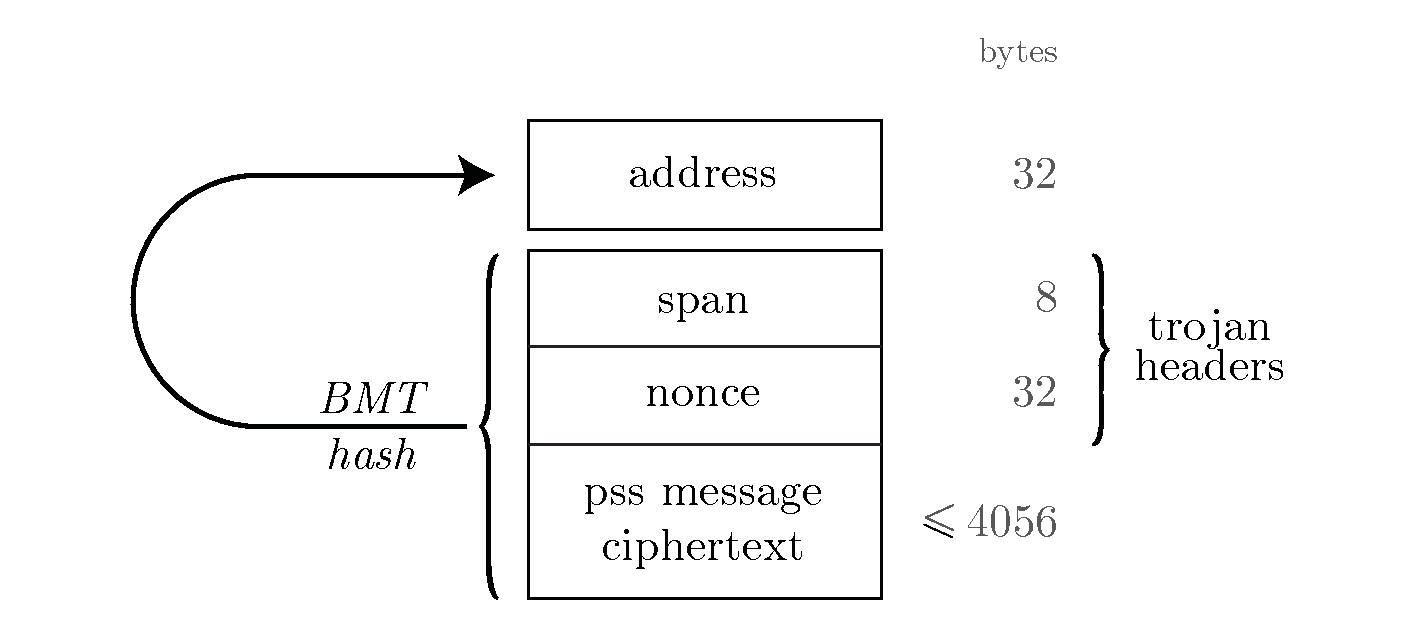
\includegraphics[width=\textwidth]{fig/trojan-chunk-2.pdf}
\caption[Trojan Chunk\statusyellow]{Trojan Chunk}
\label{fig:trojan-chunk}
\end{figure}

Knowing the public key of the recipient, sender encrypts the message (after prefixing it with its hash, length, then padding it) using asymmetric encryption. Then sender tries to find a random nonce so that when prepended to the payload, it hashes to an address that falls in the neighbourhood of the recipient based on the overlay address derived from the public key%
%
\footnote{Alternative overlays can be associated with a public key, and several public keys can be listened on by a node at a particular address.}
%
(see \ref{spec:format:bzzaddress}). The sender then uploads the resulting chunk to Swarm with postage stamps of their choice which then ends up being synced to the recipient address' neighbourhood. If the recipient node is online they receive the chunk for certain if they are the closest node. 

\subsubsection{Receiving trojan messages}

The recipient knows that a chunk is such a trojan message if and when they try to open the message with the private key corresponding to the base account's public key and then verify the integrity by hashing the payload and checking the hash against the integrity protection field of the message. Nodes that want to receive such trojan messages will keep trying to open all messages that they are closest to.

Note that forwarding nodes (or anyone else apart from sender and recipient) has no way to distinguish between a random encrypted chunk and the trojan, effectively obfuscating the message.  

\subsubsection{Mailboxing for asynchronous delivery}

If the recipient is not online the chunk will prevail as any other chunk would depending on the postage stamp it has. Whenever the recipient node comes online, it pull-syncs from the neighbourhood the chunks closest to it, among them all the trojan chunks. In other words trojan messages automatically provide \emph{mailboxing} functionality, i.e., 
without any further action needed from sender, undelivered messages are preserved and available to the recipient whenever they come online. The duration of mailboxing is controlled with the postage stamps exactly the same way as, in fact, indistinguishable from, the persistence of chunks. 

\subsubsection{Mining for proximity}

The process of finding a hash close to the recipient address is analogous to mining blocks on the blockchain. The nonce segment in a trojan chunk also plays exactly the same role as a block nonce: it provides sufficient entropy to guarantee a solution. The difficulty of mining corresponds to the minimum proximity order required to ensure that the recipient will receive the message and needs to be higher than the neighbourhood depth of the recipient%
%
\footnote{It makes sense to use the postage lottery batch depth (see \ref{sec:postage-lottery}) as a heuristic for the target proximity order when mining a trojan chunk.}
%
when it comes online, so it is logarithmic in the number of nodes in the network. The expected number of nonces that need to be tried per trojan message before an appropriate content address is found is exponential in the difficulty, and therefore equal to the number of nodes in the network. As the expected number of computational cycles needed to find the nonce equals the network size, in practice, mining a trojan will never be prohibitively expensive or slow even for a single node. The small delay in the second range is expected only at a billion nodes and even that is acceptable given that trojan messages are meant to be only for one-off initiations of a channel. All subsequent real-time exchange will happen using the bidirectional outbox model using single-owner chunks.


\subsubsection{Anonymous mailbox}

Asynchronous access to pss messages is guaranteed if the postage stamp has not yet expired. The receiver only needs to  create a node with an overlay address corresponding to the account advertised to be the recipient.    

If this turns out to insecure against targeted attacks, one can also just have an anonymous mailbox. Anonymous mailbox can receive pss messages on behalf of a client and then publish those on their feed so  that the intended recipient can read them whenever they come online.

\subsubsection{Register for aggregate indexing}

As mentioned in \ref{sec:indexing-schemes},  aggregate indexing services help nodes in monitoring sporadic feeds. For instance, a forum indexer aggregates the contribution feed of registered members. For public forums, off-chain registration  is possible and can be done by sending a pss message to the aggregator. 


\subsection{Initial contact for key exchange\statusgreen}\label{sec:pss-key-exchange}


Encrypted communication require a handshake to agree on initial parameters. The \gloss{extended triple Diffie--Hellmann Key Exchange} (\gloss{X3DH}) is such a  protocol \cite{marlinspike2016x3dh} and is used to establish the initial parameters for post-handshake communication protocol such as the double ratchet introduced for feeds (see \ref{sec:feed-as-channel}). 
Zero leak communication can be achieved by first performing a X3DH then follow the double ratchet protocol for encryption as well as indexing to retrieve the updates of the outbox feed.
In what follows, we describe how the X3DH protocol can be implemented with pss in a serverless setting. 

Swarm's X3DH uses the same primitives as customary in Ethereum, i.e., secp256k elliptic curve, keccak256 sha3 hash, and 64-byte encoding for public keys.

The Swarm X3DH protocol is set out to allow two parties to establish a shared secret that is input to post-handshake two-way messaging. The initiator is the party that initiates a two-way communication with the responder. Responder is supposed to advertise the information necessary for parties not known to the responder to call them.

X3DH uses the following keys:%
%
\footnote{The protocol specifies a one-time prekeys for callee but they can be safely ignored since they only serve  as replay protection, which is solved with other means here.}

\begin{itemize}
\item responder long-term identity key
\item responder signed prekey
\item initiator long-term identity key
\item initiator ephemeral key
\end{itemize}{}

A \gloss{prekey bundle} consists of all information the initiator needs to know about responder. Instead of servers, this info is stored in Swarm. The long-term identity address is used to construct an epoch-based feed with the topic for "prekey bundle". The latest update payload is the signed prekey's public key. The signature in the feed update chunk is signing off on the prekey. And the public key that you get from the signature gives you the public identity key's public key.%
% 
\footnote{Replacing mutual authentication based on the DH1 and DH2 values with the signature from the identity keys would reduce deniability.}
%
For human-friendly identity management, ENS can be used, with the owner of the ENS corresponding to is the owner of the prekey bundle feed. Responder's identity registered on ENS is considered authenticated.

According to the protocol,  initiator sends an initial message to responder. In swarm, this is done with trojan chunks and pss. If responder’s initial message does not use a one-time prekey, the initial message can in theory be re-sent by third party and lead the responder to assume genuine repeated requests. Such protocol replay attacks are eliminated if the post-handshake protocol adds random key material coming from the responder. 

But the initial trojan message can also be required to contain a unique identifier, e.g., the nonce used for mining. Reusing the id is not possible since it leads to
the same chunk.

In order to invite responder to an outbox-feed based private communication channel, the initiator looks up the respnder's public prekey bundle,  generates the triple Diffie-Hellmann shared secret, see figure \ref{fig:x3dh}.


\begin{figure}[htbp]
   \centering
   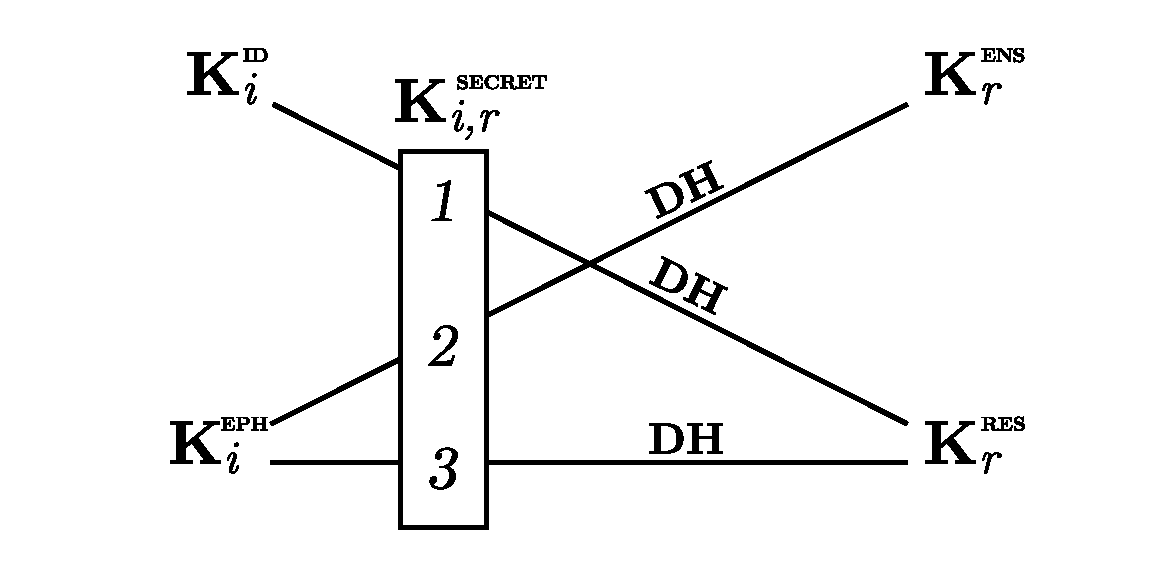
\includegraphics[width=.7\textwidth]{fig/x3dh.png}
   \caption[X3DH initial message \statusorange]{X3DH initial message}
   \label{fig:x3dh}
\end{figure}


\subsection{Addressed envelopes\statusgreen}\label{sec:addressed-envelopes}

\subsubsection{Mining single-owner chunk addresses}
The question immediately arises whether it makes sense to somehow mine single-owner chunks. Since the address in this case is the hash of a 32 byte id and a public key, the id provides enough entropy even for a fixed public key to mine arbitrary addresses. Since the address can be mined before the chunk content is associated with it, it can serve as an \gloss{addressed envelope}. If we mine an id for a public key so that the resulting single-owner chunk address is close to a target overlay address and we give it to the owner of the corresponding private key, we effectively allow them to send a message to the target without computation. All they need to do is when they wish to send a message to the target, they create a trojan message and sign it under the premined address. If they sign with the private key corresponding to the public key that is used in the address, the chunk will be valid.

\subsubsection{Pre-paid postage}

These chunks behave the same way as normal trojan messages, their privacy properties being the same if not somewhat better since issuer/recipient can associate a random public key with which the message is encrypted, or even use symmetric encryption for speed. If postage stamp is prepaid on the address and given to the sender, they can push-sync the chunk to the target without them needing to pay. Such a construct effectively implements \emph{addressed envelopes with prepaid postage} and serves as a  base layer solution for various high-level communication needs: 1) push notifications about an update to subscribers without computational or monetary burden on the publisher 2) free contact vouchers 3) no delay direct message response.  

Issuing a prepaid addressed envelope involves the following process:

\begin{enumerate}
\item \emph{assume} issuer $I$, prospective sender $S$, and prospective recipient $R$ with public keys $P_I, P_S, P_R$ and overlay addresses $A_I, A_S, A_R$
\item \emph{mine} -- $I$ finds a nonce $N_R$ such that when used as an index for single-owner chunk address hashes to $H_R$ which is in the nearest neighbourhood of $A_R$
\item \emph{pay postage} -- $I$ signs $H$ to produce a witness for an appropriate postage payment to produce stamp $PS_R$ 
\item \emph{encapsulate} -- package $N_R$ and $PS_R$ as the prepaid addressed envelope $E$ 
% and encrypt it with $P_S$ then wrap it as a trojan message
% \item \emph{mine} -- find a nonce $N_S$ such that the trojan chunk hashes to $H_S$ which is in the nearest neighbourhood of $A_S$. 
\end{enumerate}

\subsubsection{Using and opening a pre-paid addressed envelope}

Prospective sender $S$ is assumed to receive a prepaid envelope $E$ and carries out  the following steps:
\begin{enumerate}
    \item \emph{decrypt} message with the private key belonging to $P_S$
    \item \emph{deserialise} unpack and identify $PS_R$ and $N_R$, extract $H_R$ from $PS_R$
    \item \emph{verify} postage stamp $PS_R$ as well as check if $N_R$+$P_S$ hashes to $H_R$ to make sure address belongs to  $S$.
    \item \emph{store} $N_R$, $PS_R$ 
\end{enumerate}

When sender wants to use the envelope to send message $M$ to $R$ (potentially unknown to sender), they 
follow the steps:

\begin{enumerate}
\item \emph{encrypt} the message content $M$ as payload with $P_R$ and wrap it as a trojan message $T$
\item \emph{hash} the encrypted trojan message resulting in $H_T$
\item \emph{sign} $H_T$ using $N_R$ as salt with the private key belonging to $P_S$ producing signature $W$
\item \emph{encapsulate} nonce $N_R$ as id, the signature $W$ and the trojan message $T$ as payload in a valid single-owner chunk with address $H_R$
\item \emph{post} the chunk with the valid stamp $PS_R$
\end{enumerate}


When $R$ receives chunk with address $H_R$

\begin{enumerate}
\item \emph{verify} postage stamp $PS_R$ and validate the chunk as a single-owner chunk with payload $T$.
\item \emph{decrypt} $T$ with the private key belonging to $P_R$
\item \emph{deserialise} plaintext as trojan message, identify message payload $M$ and check its integrity with the hash field
\item \emph{consume} $M$
\end{enumerate}

% \subsubsection{Subscribe to publisher}
If $I$ wants to subscribe $R$ to the next activity on a channel $C$ published by $S$, it needs to give $S$ the prepaid addressed envelope as a trojan message to $A_S$.
If $I=R$, the $I$ subscribe themselves.

\subsection{Update notification requests\statusgreen}\label{sec:update-notification-requests} 

Now consider the use case when a publisher does not want to receive direct messages or send out notifications. Is there a way for consumers to "plant" a notification request at the address of the update directly? The challenge is that (prepaid) addressed envelopes so far required that the sender's public key is known, so that they can produce a valid single-owner chunk for the response. In this section, we show another technique which allows for the case when sender has not revealed their overlay or refuse to handle notifications.                                                                                                                                                                                                                               
\subsubsection{Requesting update} 

If $I$  wants to subscribe $R$ to a  particular update at address $H_U$ derived from $I_U$ and $P_U$, it takes $I_U$ as a private key $K_U$ and corresponding public key $P_U$. It also chooses a random salt $S_U$ and hashes it with $I_U$ to result in a private key $K_{SU}$ and corresponding public key $P_{SU}$. Then mine a single-owner address $H_{SU}$ for $P_{SU}$ with nonce $N_{SU}$ that is close to the recipient address $A_R$ and prepare it as a prepaid addressed envelope. Package the envelope together with the salt $S_U$, encrypt it with $P_U$ as a trojan message and
package it as a trojan chunk with nonce $N_U$ so that the resulting content hash $H_N$ falls in the neighbourhood of $H_U$ or in fact arbitrarily close to $H_U$. This chunk is called \gloss{update notification request} and issuer sends it with a postage stamp so that nodes in the proximity of $H_U$ can store it.


\subsubsection{Sending the update notification}

When a node in the proximity of $H_U$ receives the desired update chunk, a single-owner chunk with address $H_U$, it tries to find matching update notification requests for it. In order not to need to try with every chunk, issuer mines the request chunk to be arbitrarily close to $H_U$ so that notifiers only need to iterate over a small number of nearest chunks in their local storage. To find the corresponding requests, matching chunks are taken as trojans with payload to be decrypted with the index $I_U$ extracted from the incoming update chunk used as a private key. The resulting trojan is verified, its payload is deserialised and postage stamp $PS_R$ and salt $S_U$ are extracted from it. Then the salt is used to derive private key $K_{SU}$ with which the actual notification (the content of the incoming update chunk with index and publisher signature) is signed, then create the valid single-owner chunk with nonce $N_{SU}$ as index, the signature and the actual notification as payload at address $H_{SU}$. The node then sends this chunk, called \gloss{update notification} alongside the corresponding postage stamp not knowing anything of the recipient's identity or anything about the channel the update was on.


\subsubsection{Receiving the notification}

When $R$ receives the notification chunk at address $H_{SU}$, it validates as a single-owner chunk and the update chunk content is extracted. If valid, save the update chunk and call the handler for channel index $I_U$.
If $I=R$, issuer and recipient are the same, then this is a notification request to issuer as recipient.
Typically, the issuer has requested update at $H_U$, then after time-out, the notification request is created and sent but the database has an open request for $H_U$. When it receives the notification from the node that is in the proximity of $H_U$, the chunk is validated, saved and triggers the handler(s).


\subsubsection{Features}

\begin{itemize}
    \item originator does not need to know public key of any particular node in the neighbourhood of the update
    \item originator does not need to rely on any node to be online
    \item notifier needs to have both the update chunk as well as the notification to write the notification chunk
    \item mining the notification request address in close proximity of the update chunk's address allows notifiers to look up the notification request more efficiently
    \item notification request is not distinguishable from a random single-owner chunk
    \item forwarding nodes cannot change or interpret the notification 
    \item notifier knows nothing about originator or notified peers
\end{itemize}

nvmvh b 